\documentclass[a4paper, 12pt, oneside]{article}
\usepackage[utf8]{inputenc}
\usepackage[margin=3cm, bindingoffset=1cm]{geometry}
\linespread{1.5}
\usepackage{float}
\usepackage{csquotes}
\usepackage{subfig}
\usepackage{graphicx}
\usepackage{indentfirst}
\usepackage{fancyhdr}
\usepackage{alphabeta}
\usepackage{algpseudocode}
\usepackage{algorithm}
\usepackage{hyperref}
\usepackage[T1]{fontenc}
\usepackage{listings}
\usepackage[htt]{hyphenat}
\usepackage{pgfplots}

\usepackage[
    backend=biber,
    sorting=none
]{biblatex}
\addbibresource{bibliography.bib}


\setlength{\parindent}{1cm}

\pagestyle{fancy}
\fancyhf{}
\fancyhead[C]{\textbf{\leftmark}}
\fancyfoot[C]{\thepage}
\renewcommand{\headrulewidth}{1pt}
\renewcommand{\footrulewidth}{1pt}
\renewcommand{\contentsname}{Indice}
\renewcommand{\figurename}{Fig.}

\usepackage[Conny]{fncychap}

  
\begin{document}
\begin{titlepage}
    \begin{center}
        \LARGE{\uppercase{Università degli Studi di Salerno}}\\
        \vspace{5mm}
    	\uppercase{\normalsize Dipartimento di Informatica }\\
    \end{center}
    \begin{figure}[H]
        \centering
        
\includegraphics[width=0.35\textwidth]{logo_unisa}
    \end{figure}
    
    \begin{center}
        \normalsize{Corso di \textbf{Penetration Testing and Ethical Hacking}}\\
    	\vspace{10mm}
    	\LARGE{\textbf{\textsc{NoobBox-1}:\\ Metodologie Utilizzate per il processo di Penetration Testing}}\\
    	\vspace{3mm}
        \large{\uppercase{Anno Accademico 2022/2023}}
    \end{center}

    \vspace{55mm}
    \noindent
    \begin{minipage}[t]{0.6\textwidth}
    	\textsc{Docente}:\\\textbf{Prof. Arcangelo Castiglione}
    	\vspace{10mm}\\
    \end{minipage}
    \hfill
    \begin{minipage}[t]{0.4\textwidth}\raggedleft
    	\textsc{Studente}: \\\textbf{Hermann Senatore}
    \end{minipage}
\end{titlepage}

\tableofcontents
\newpage

\section{Introduzione}
Questo documento si propone di raccogliere in maniera esaustiva tutte le operazioni che sono state compiute allo scopo di condurre l'analisi sull'asset vulnerabile \textsc{NoobBox-1}, disponibile sulla piattaforma VulnHub \cite{noobbox} e che fa uso di un sistema operativo \textbf{GNU\slash Linux}.

Tale documento costituisce il \textbf{Documento 2}, necessario per la consegna dell'attività progettuale del corso di \textbf{Penetration Testing and Ethical Hacking} ed assicura la \textbf{replicabilità} dell'intero processo sulla piattaforma utilizzata.

In particolare, questa sezione consiste una panoramica sull'asset che è stato analizzato e ci si sofferma sull'ambiente utilizzato per condurre l'analisi sull'asset stesso.

\subsection{Ambiente di lavoro ed Information Gathering}
La piattaforma sulla quale è stato svolto l'intero processo consiste in un \textbf{MacBook Air} (late 2020) che utilizza il processore Apple Silicon M1 e che fa uso dell'architettura \textbf{arm64} (aka \textbf{aarch64}).

Per condurre concretamente l'indagine sono state sfruttate due macchine virtuali utilizzando l'\textit{hypervisor} \textbf{UTM}, che utilizza \textbf{QEMU} come suo backend.

In particolare:

\begin{itemize}
    \item La prima macchina virtuale consiste nella versione \textbf{aarch64} del sistema operativo \textbf{Kali Linux};
    \item La seconda macchina virtuale consiste invece nell'asset vulnerabile menzionato poc'anzi.
\end{itemize}.

Di seguito sono presenti alcuni dettagli su entrambe le macchine.

\subsubsection{Macchina virtuale 1: dettagli}
La prima macchina virtuale è stata creata in maniera standard utilizzando l'immagine ISO reperibile presso il sito web della distribuzione \cite{kali}. La versione utilizzata risulta essere la \textbf{2023.1}, rilasciata il 13 marzo 2023. 

In fase di installazione è stato necessario adottare alcuni accorgimenti suggeriti nella relativa documentazione dell'\textit{hypervisor} utilizzato \cite{kali-utm}. Le informazioni presenti in questa pagina sono state create per le versioni \textbf{2022.x} ma sono valide anche per la versione utilizzata durante questo processo.

La macchina virtuale in questione utilizza il kernel Linux 6.1 e di seguito è presente l'output del comando \verb|uname -a|.

\begin{figure}[h]
    \centering
    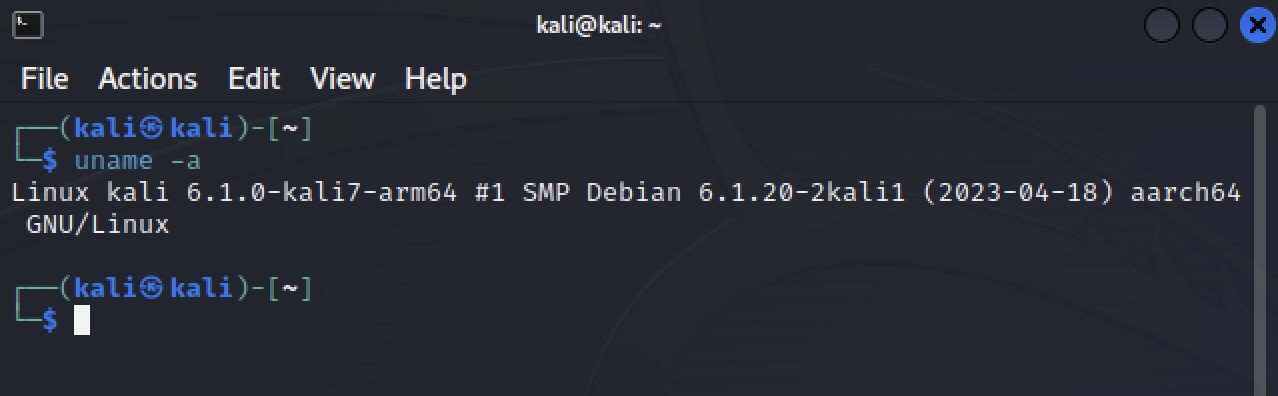
\includegraphics[scale=0.5]{img/uname.png}
    \caption{La versione del kernel utilizzata da Kali}
\end{figure}

\subsubsection{Dettagli sull'asset}
Come menzionato in precedenza, la seconda macchina consiste proprio nell'asset su cui deve essere condotta l'analisi. Originariamente pensato per essere una sfida CTF, sulla piattaforma VulnHub viene rivelata la presenza di due \textit{flags} a cui accedere: una per l'utente non privilegiato ed una per \texttt{root}. 

Naturalmente, allo scopo di questo progetto non ci si è limitati alla cattura delle flag ma è stato seguito un approccio più sistematico che prevede l'utilizzo di tools e di metodologie standard tipiche di un processo di Penetration Testing.

Sulla piattaforma VulnHub viene offerto il download di NoobBox-1 in formato \texttt{.ova}, compatibile con il software \textbf{Oracle VirtualBox}. Tuttavia, al momento della stesura di questo documento, non esiste una versione nativa di tale software per la piattaforma Apple Silicon in uso e l'hypervisor d'elezione non supporta l'importazione di file \texttt{.ova}. 

Di conseguenza, si è reso necessario un ulteriore step di conversione per rendere tale macchina virtuale utilizzabile con \textbf{UTM} \cite{qcow}. Tale step consiste nella conversione dell'immagine disco in formato \texttt{.vmdk} presente all'interno del file \texttt{.ova} nel formato \texttt{.qcow2}, utilizzato dal software \textbf{QEMU} e quindi da \textbf{UTM}.

Gli step seguiti per la conversione dell'immagine disco sono riportati qui di seguito:

\begin{enumerate}
    \item Installazione di QEMU in maniera \textit{system-wide} usando il package manager \textbf{Homebrew}: \verb|brew install qemu|;
    \item Conversione dell'immagine disco usando il tool \textbf{qemu-img}.
    \begin{center}
        \verb|qemu-img convert -f vmdk -O qcow2 NoobBox-disk001.vmdk NoobBox-disk.qcow2|.
    \end{center}
    Lo switch \texttt{-f} permette di esplicitare il formato \textbf{sorgente}, mentre lo switch \texttt{-O} quello di \textbf{output}.
\end{enumerate}

Successivamente, è stato possibile creare una nuova macchina virtuale \textbf{Linux} e, conseguentemente, importare il file appena creato come disco virtuale.

Al primo avvio della macchina ci si rende conto che è in uso il sistema operativo \textbf{Debian GNU\slash Linux} in versione 10 (codename \texttt{buster}), rilasciato il 6 Luglio 2019. \cite{debian}

In ogni caso, la versione del sistema operativo utilizzato dall'asset sarà oggetto di una successiva analisi per evitare qualsiasi tipo di depistaggio o ambiguità.

La quantità di informazioni che è possibile carpire senza effettuare analisi "esterne" all'asset stesso si ferma tuttavia qui poiché \textbf{non è possibile accedere alla macchina}. Lo scopo della sfida CTF è in reltà proprio quello di effettuare il login e "catturare" le due flag descritte in precedenza. È quindi necessario svolgere ulteriori analisi

Tutti i passaggi descritti in questo documento assumono che la macchina Kali si trovi \textbf{sulla stessa rete locale} della macchina che costituise l'asset da analizzare.

\section{Target Discovery}
Come detto, la diretta conseguenza dell'impossibilità di accedere all'asset in alcun modo consiste nella necessità di determinare in qualche modo il suo indirizzo IP sulla rete.

L'hypervisor UTM crea come impostazione predefinita una rete \textbf{NAT} che usa il range (qui riportato in notazione CIDR) \textbf{192.168.64.0\slash24}.

Prima di tutto, è necessario specificare che:

\begin{itemize}
    \item Anche la macchina Host (su cui è in esecuzione l'hypervisor) fa parte della rete NAT ed ha indirizzo IP \textbf{192.168.64.1} sull'interfaccia \texttt{bridge100};
    \item La macchina Kali ha come indirizzo \textbf{192.168.64.15} sull'interfaccia \texttt{eth0}.
\end{itemize}

A questo punto, per determinare l'indirizzo IP dell'asset è possibile utilizzare il tool \texttt{netdiscover}, che viene fornito di default con Kali Linux e che deve essere eseguito come utente \texttt{root}.

Suddetto tool, secondo la documentazione accessibile mediante il comando \texttt{man netdiscover}, permette di rilevare host attivi su di una rete locale inviandogli richeste \textbf{ARP}. 

Due sono le opzioni che devono essere specificate in questo contesto:

\begin{itemize}
    \item \texttt{-i eth0} permette di utilizzare l'interfaccia di rete \texttt{eth0};
    \item \texttt{-r 192.168.64.0\slash24} permette invece di specificare il range di indirizzi compreso tra 192.168.64.0 e 192.168.64.255, specificato in notazione CIDR.
\end{itemize}.

\newpage
L'output per
\begin{center}
    \texttt{netdiscover -i eth0 -r 192.168.64.0\slash24}
\end{center}

viene riportato qui di seguito.

\begin{figure}[h]
    \centering
    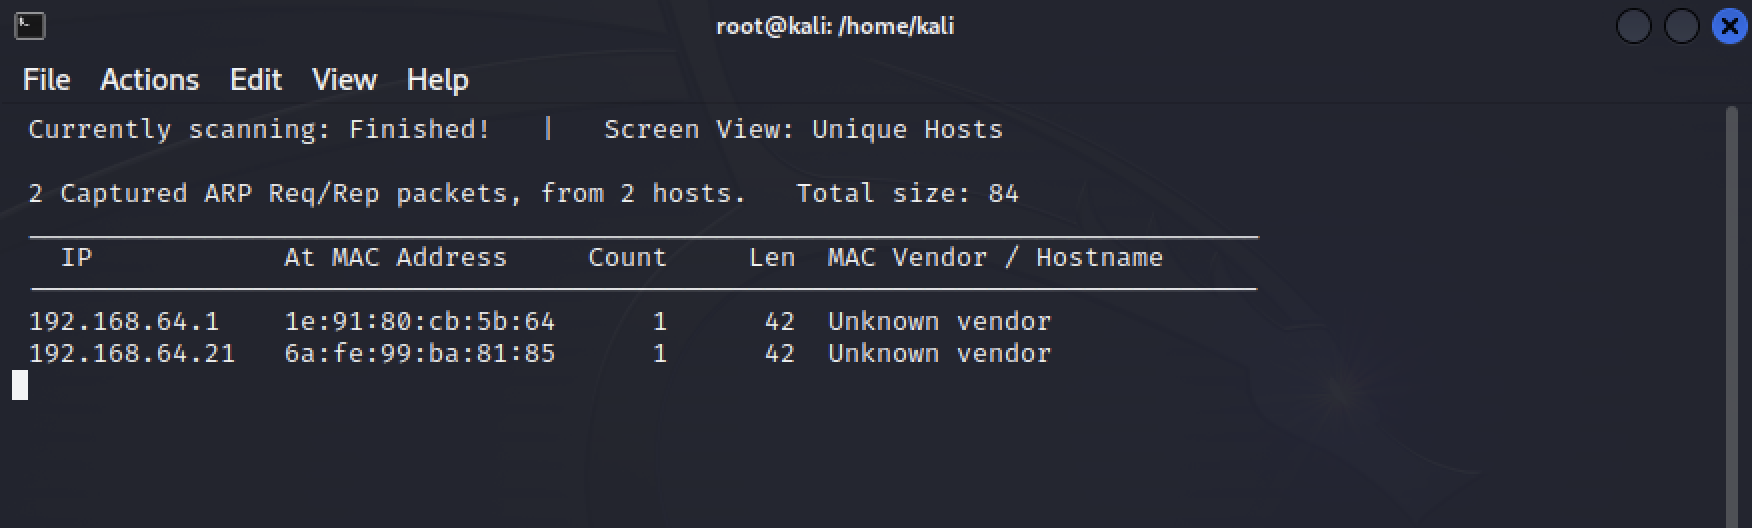
\includegraphics[scale=0.5]{img/netdiscover.png}
    \caption{L'output di \texttt{netdiscover}}
\end{figure}

Tralasciando l'host 192.168.64.1 che si è menzionato appartenere alla macchina fisica che ospita l'hypervisor, è possibile notare la presenza di un host attivo con indirizzo 192.168.64.21 e, dato che al momento dell'esecuzione del tool non erano in esecuzione altre macchine virtuali oltre all'asset in analisi, è possibile concludere che \textbf{192.168.64.21} sia effettivamente \textbf{il suo indirizzo}.

\subsection{Probing della macchina}

Una volta ottenuto l'indirizzo IP della macchina, è ora necessario cercare di capire se la macchina identificata sia effettivamente raggiungibile in qualche modo. In questa sezione, viene sfruttato il tool \texttt{ping} che sfrutta il meccanismo degli \textbf{ICMP Echo Request\slash Reply}.

La sintassi del comando ping, come specificato nella relativa documentazione, prevede la specifica di un indirizzo IP da contattare, ed eventualmente (mediante lo switch \texttt{-c}) il numero di richieste da inoltrare al target da analizzare. In questo contesto, al target verranno inoltrare 3 richieste ICMP. Il comando eseguito risulta quindi essere:

\begin{center}
    \texttt{ping -c 3 192.168.64.21}
\end{center}

\begin{figure}[h!]
    \centering
    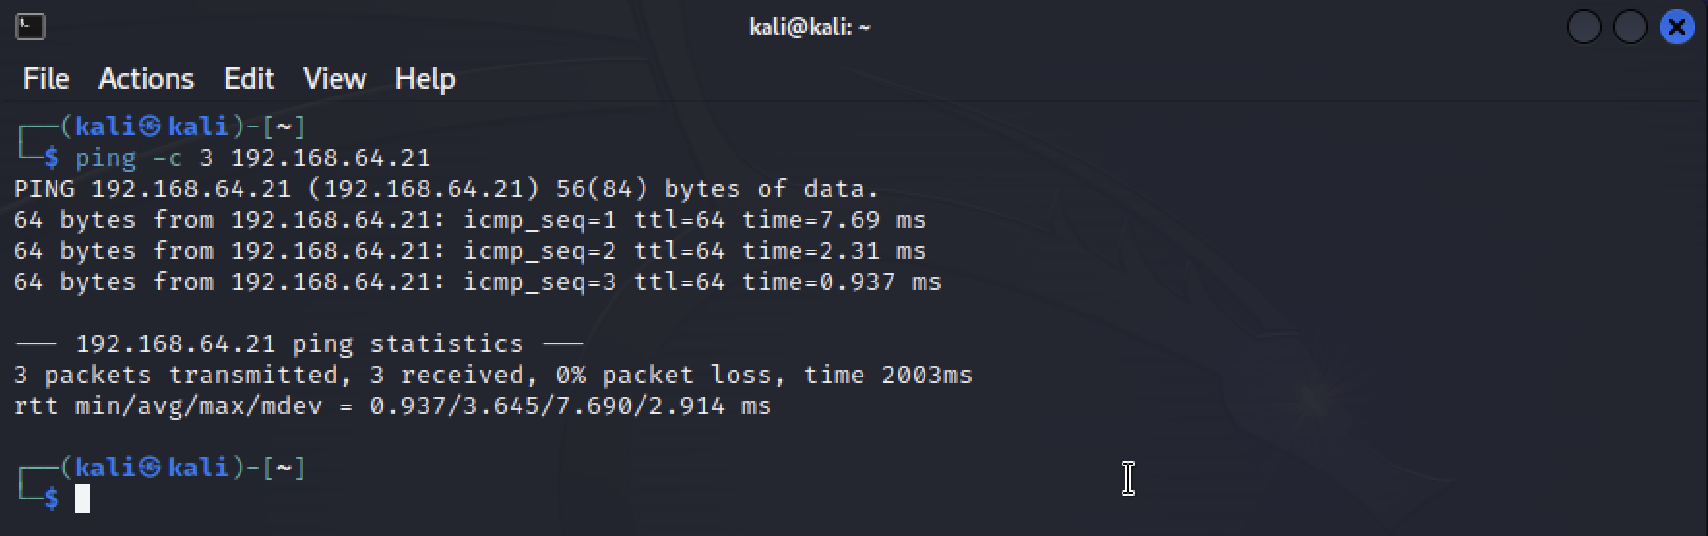
\includegraphics[scale=0.5]{img/ping.png}
    \caption{L'output di \texttt{ping}}
\end{figure}

Senza adottare particolari accorgimenti, dall'output del comando mostrato qui sopra è possibile notare come la macchina in questione sia effettivamente \textbf{raggiungibile dall'esterno}, almeno utilizzando il protocollo ICMP.

\subsection{OS Fingerprinting}
Il passo successivo dell'analisi condotta consiste nell'identificare con certezza ed in maniera non ambigua il sistema operativo utilizzato dall'asset. A questo scopo, è possibile far riferimento ai tool \texttt{p0f} ed \texttt{nmap}, quest'ultimo utilizzato anche nelle fasi successive dell'analisi.

\subsubsection{\texttt{p0f}}
Il tool \textbf{\texttt{p0f}} utilizza una \textbf{tecnica di fingerprinting} basata sull'analisi della composizione dei pacchetti \textbf{TCP\slash IP} provenienti dalla macchina target per determinare \textbf{passivamente} il suo sistema operativo\cite{p0f}. L'utilizzo del tool prevede l'esecuzione come utente root. Una volta avviato, si mette in ascolto sull'interfaccia specificata dallo switch \texttt{-i} (in questo caso \texttt{eth0}), catturerà i pacchetti e restituirà informazioni sull'host che ha generato quel determinato pacchetto. Si rivela quindi necessaria la \textbf{generazione} di traffico verso il target per condurre l'analisi in questione. 

Il comando completo utilizzato in questo contesto risulta essere:

\begin{center}
    \texttt{p0f -i eth0}
\end{center}

Come prima cosa, si è provato ad accedere all'asset mediante il comando \texttt{curl} utilizzando l'indirizzo IP ottenuto in precedenza sulla porta 80, che in questo caso si è rivelata \textbf{aperta}.\footnote{Si tenga presente che lo stato della porta 80 costituisce già di per sé un elemento \textbf{prezioso} per l'indagine in corso, ma una discussione approfonditta su questo topic verrà affrontata nella sezione dedicata alla \textbf{Target Enumeration}}.


Analizzando tuttavia i risultati mostrati a schermo (qui di seguito, si notino i punti interrogativi in corrispondenza della voce \texttt{server}) ci si accorge che il tool \texttt{p0f} \textbf{non è riuscito ad identificare correttamente il sistema operativo del target}. Si è reso quindi necessario provare altre strategie.

\begin{figure}[h!]
    \centering
    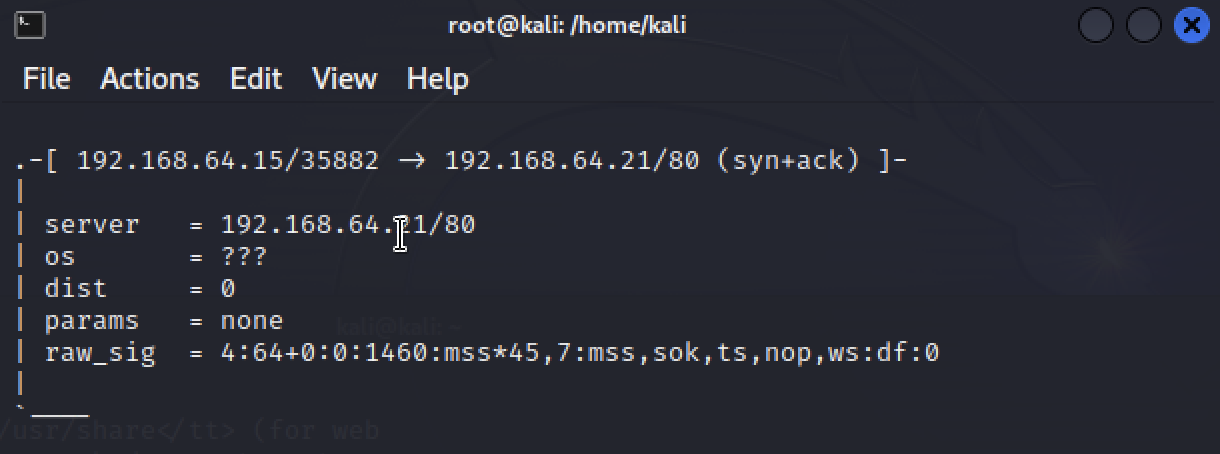
\includegraphics[scale=0.5]{img/p0f.png}
    \caption{L'output di \texttt{p0f}. L'indirizzo IP \texttt{192.168.64.15} appartiene alla macchina Kali.}
\end{figure}

\subsubsection{\texttt{nmap}}
\texttt{nmap} è probabilmente uno dei tool più conosciuti ed utilizzati per condurre operazioni di Target Enumeration (ed infatti verrà utilizzato principalmente in questa fase per effettuare l'operazione di \textbf{port scanning}) e di security auditing in generale ma che può essere utilizzato anche per effettuare OS Fingerprinting.\cite{nmap}

Suddetta operazione può essere effettuata mediante lo switch \texttt{-O} in combinazione con l'host da scansionare. La command line completa utilizzata in questo caso è la seguente:

\begin{center}
    \texttt{nmap -O 192.168.64.21}
\end{center}

Di seguito viene riportato il risultato della scansione.

\begin{figure}[h!]
    \centering
    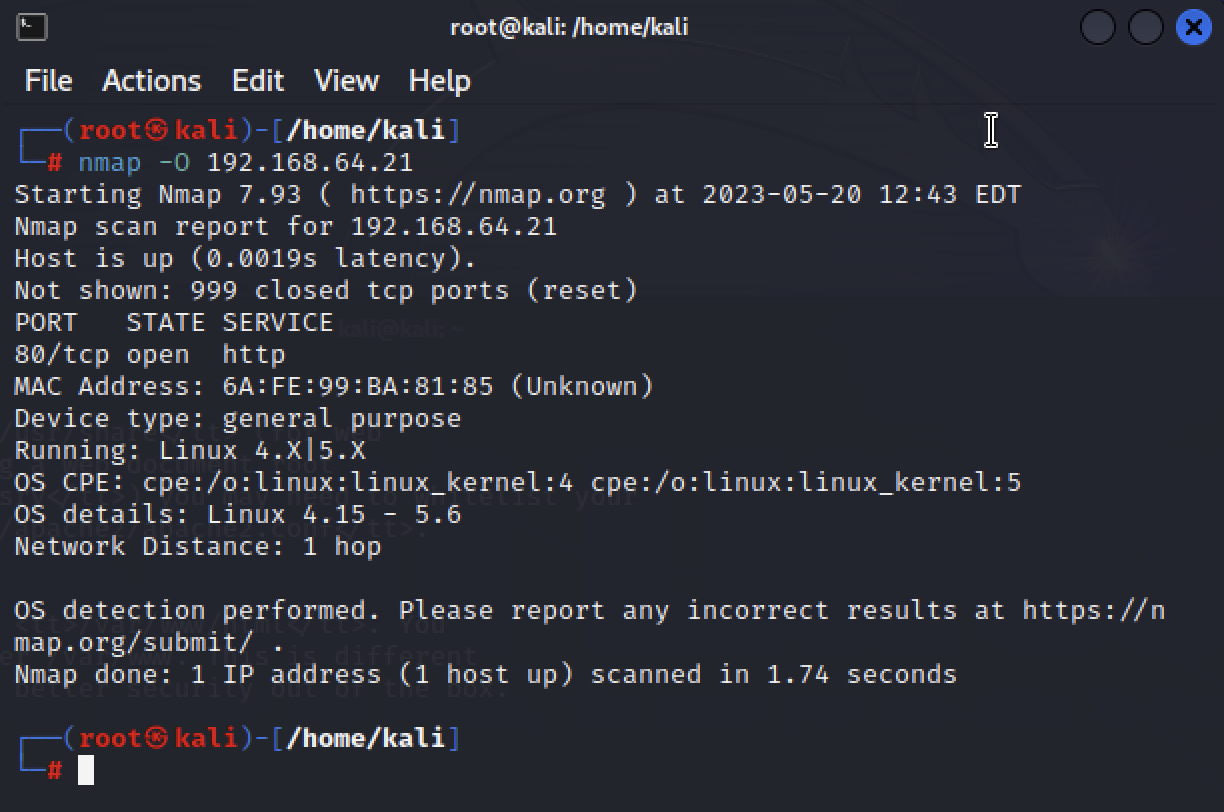
\includegraphics[scale=0.5]{img/nmap-os.png}
    \caption{L'output di \texttt{nmap}.}
\end{figure}

Secondo \texttt{nmap}, il target consiste in una macchina \textbf{general purpose} che utilizza il kernel \textbf{Linux} in una versione compresa tra la \textbf{4.15} e la \textbf{5.6}. Considerando che Debian 10 è stato rilasciato con il kernel \textbf{4.19} \cite{debian}, è possibile concludere che le informazioni ottenute in precedenza risultano \textbf{corrette}. Si noti come \texttt{nmap} abbia inoltre rilevato la porta 80 come \textbf{aperta}.

\section{TCP Port Scanning e Target Enumeration}

Nella fase precedente, oltre all'estrazione di diverse informazioni sul target, è stata ricavata anche un'altra, importante, informazione circa lo stato di apertura della porta \texttt{tcp/80}. Il fatto che la porta 80 sia aperta fa presupporre che sul target sia in esecuzione un qualche tipo di servizio web. Questa sezione, definita di \textbf{Target Enumeration}, approfondisce questa ipotesi e conduce un'analisi sistematica riguardo ai servizi in esecuzione sul target mediante il tool \texttt{nmap}, stavolta utilizzato nel suo contesto principale.

In particolare, il tool \texttt{nmap} sarà utilizzato per:

\begin{itemize}
    \item Scansionare tutte le 65535 porte del target (switch \texttt{-p-});
    \item Identificare la versione dei servizi attivi (switch \texttt{-sV});
    \item Esportare i risultati della scansione in formato XML nel file \texttt{nmap\_noobbox\_report.xml} (switch \texttt{-oX nmap\_noobbox\_report.xml}).
\end{itemize}

Il comando utilizzato quindi risulta essere:

\begin{center}
    \texttt{nmap -p- -sV 192.168.64.1 -oX nmap\_noobbox\_report.xml}
\end{center}

In questo caso, avendo a disposizione l'accesso root alla macchina Kali, è stato utilizzata la cosiddetta \textbf{SYN Scan} (switch \texttt{-sS}, ma che essendo la scansione di default è stato omesso dalla command line).

Di seguito è riportato l'output del tool.

\begin{figure}[h!]
    \centering
    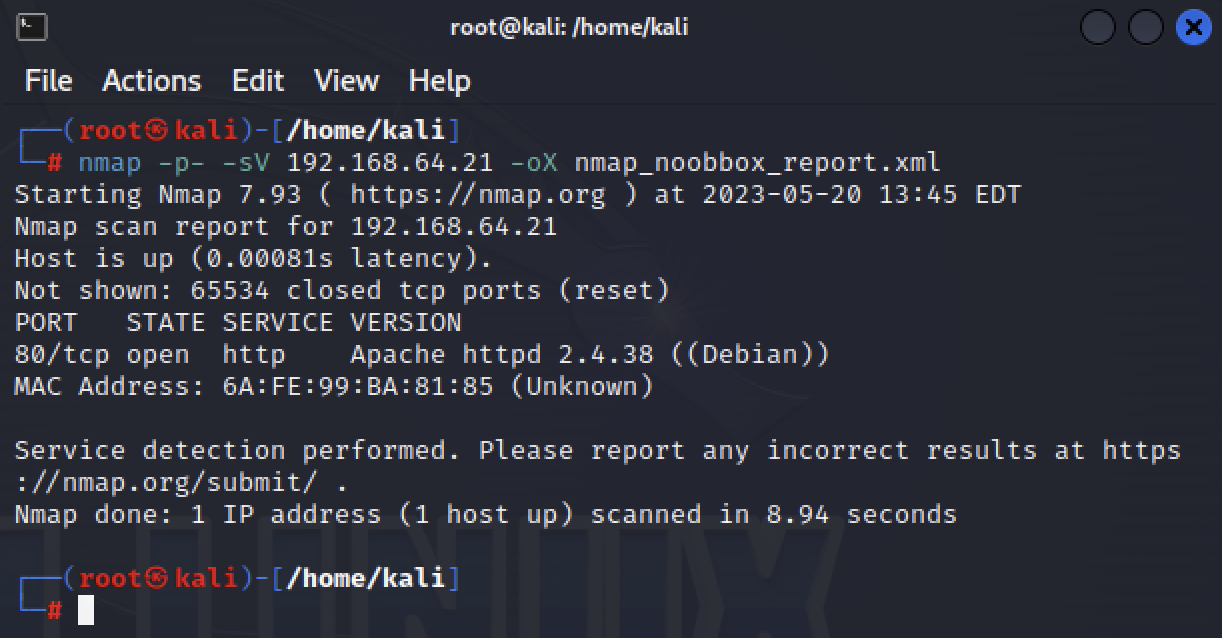
\includegraphics[scale=0.5]{img/nmap-enum.png}
    \caption{L'output di \texttt{nmap}.}
\end{figure}

In allegato al presente documento è presente il report generato da \texttt{nmap} e convertito in HTML mediante il tool \texttt{xsltproc}, chiamato \texttt{nmap\_noobbox\_report.html}.

\subsection{TCP Port Scanning: Analisi dei risultati}
Facendo riferimento al report generato è possibile notare che:

\begin{itemize}
    \item Il servizio presente sulla porta 80 TCP (identificata come aperta anche in precedenza) consiste in \textbf{Apache \texttt{httpd}} in versione \textbf{2.4.38};
    \item Non è presente nessun altro servizio TCP attivo sul target, dato che le altre 65534 porte sono state dichiarate \textbf{chiuse};
    \item È stato possibile ottenere un ulteriore discontro sul sistema operativo in esecuzione sull'asset: \textbf{Debian}.
\end{itemize}

\subsection{Extra: UDP Port Scanning}
La scansione effettuata in precedenza tramite \texttt{nmap} ha determinato lo stato di apertura delle 65535 porte \textbf{TCP}. Per completezza, sarà ripetuta la stessa scansione delle 65535 porte stavolta usando il protocollo \textbf{UDP}. Il tool utilizzato in questo contesto consiste in \texttt{unicornscan}. Questo tool non è presente nell'installazione di default di Kali Linux, ma è possibile installarlo (insieme alle relative dipendenze) mediante il comando:

\begin{center}
    \texttt{sudo apt install unicornscan}
\end{center}

La sintassi di \texttt{unicornscan} \cite{unicornscan} è abbastanza simile a quella utilizzata da \texttt{nmap}. In questo caso, il tool verrà utilizzato per:

\begin{itemize}
    \item Effettuare una scansione \textbf{UDP} (switch \texttt{-m U});
    \item Scansionare le 65535 porte dell'asset con indirizzo IP 192.168.64.21 (usando la sintassi \texttt{192.168.64.21:1-65535});
    \item Ottenere un output \textit{prolisso} (switch \texttt{-Iv});
    \item Inviare 2000 pacchetti al secondo (più veloce rispetto ai 300 pacchetti al secondo di default) (switch \texttt{-r 2000}).
\end{itemize}

Riassumendo:

\begin{center}
    \texttt{unicornscan -m U 192.168.64.21:1-65535 -Iv -r 2000}
\end{center}

Di seguito viene riportato l'output del comando precedente.

\begin{figure}[h!]
    \centering
    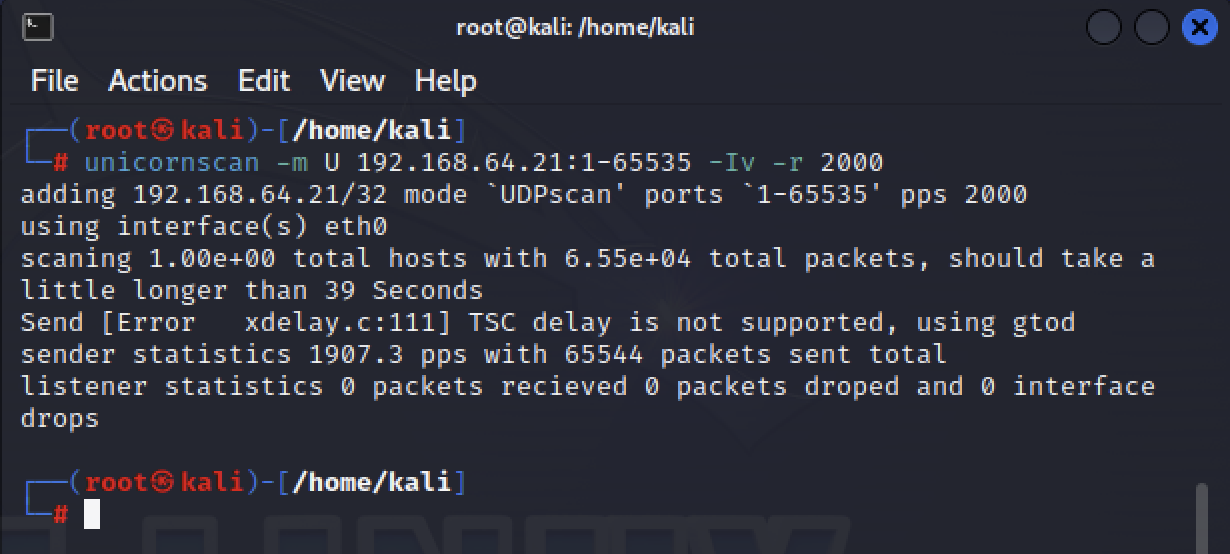
\includegraphics[scale=0.5]{img/unicornscan.png}
    \caption{L'output di \texttt{unicornscan}.}
\end{figure}

\subsubsection{UDP Port scanning: analisi dei risultati}
Consultando l'output del comando, ci si rende conto che sull'asset \textbf{non sia presente} alcun servizio attivo su \textbf{nessuna} porta UDP.

Si noti il messaggio di errore relativo al delay. Secondo la \textit{manpage} \cite{unicornscan-man} del tool, il tool di default sfrutta il timer \textbf{TSC} per gestire il delay tra l'invio dei vari pacchetti. Quando questo timer non è disponibile, il tool ne utilizza un altro: \textbf{GTOD}. 

Il timer TSC è presente su quasi tutte le CPU \textbf{x86} ed \textbf{x86\_64} con quella denominazione, ma non sulle CPU basate sull'architettura \textbf{aarch64}, come quella utilizzata per condurre l'indagine. 

La scansione con \textbf{unicornscan} ha quindi utilizzato il timer \textbf{GTOD}, senza particolari differenze all'atto pratico.

\subsection{Analisi del server web}
Uno dei risultati principali della fase di port scanning consiste nell'aver scoperto che la porta 80 sia \textbf{aperta}. Dall'analisi condotta mediante \texttt{nmap} è stato appurato che sulla porta 80 sia attivo il web server \textbf{Apache \texttt{httpd}}. 

Visitando la pagina \texttt{http://192.168.64.21/} dalla macchina Kali, viene infatti presentata la pagina di default del web server quando installato su \textbf{Debian}.
\newpage

\begin{figure}[h!]
    \centering
    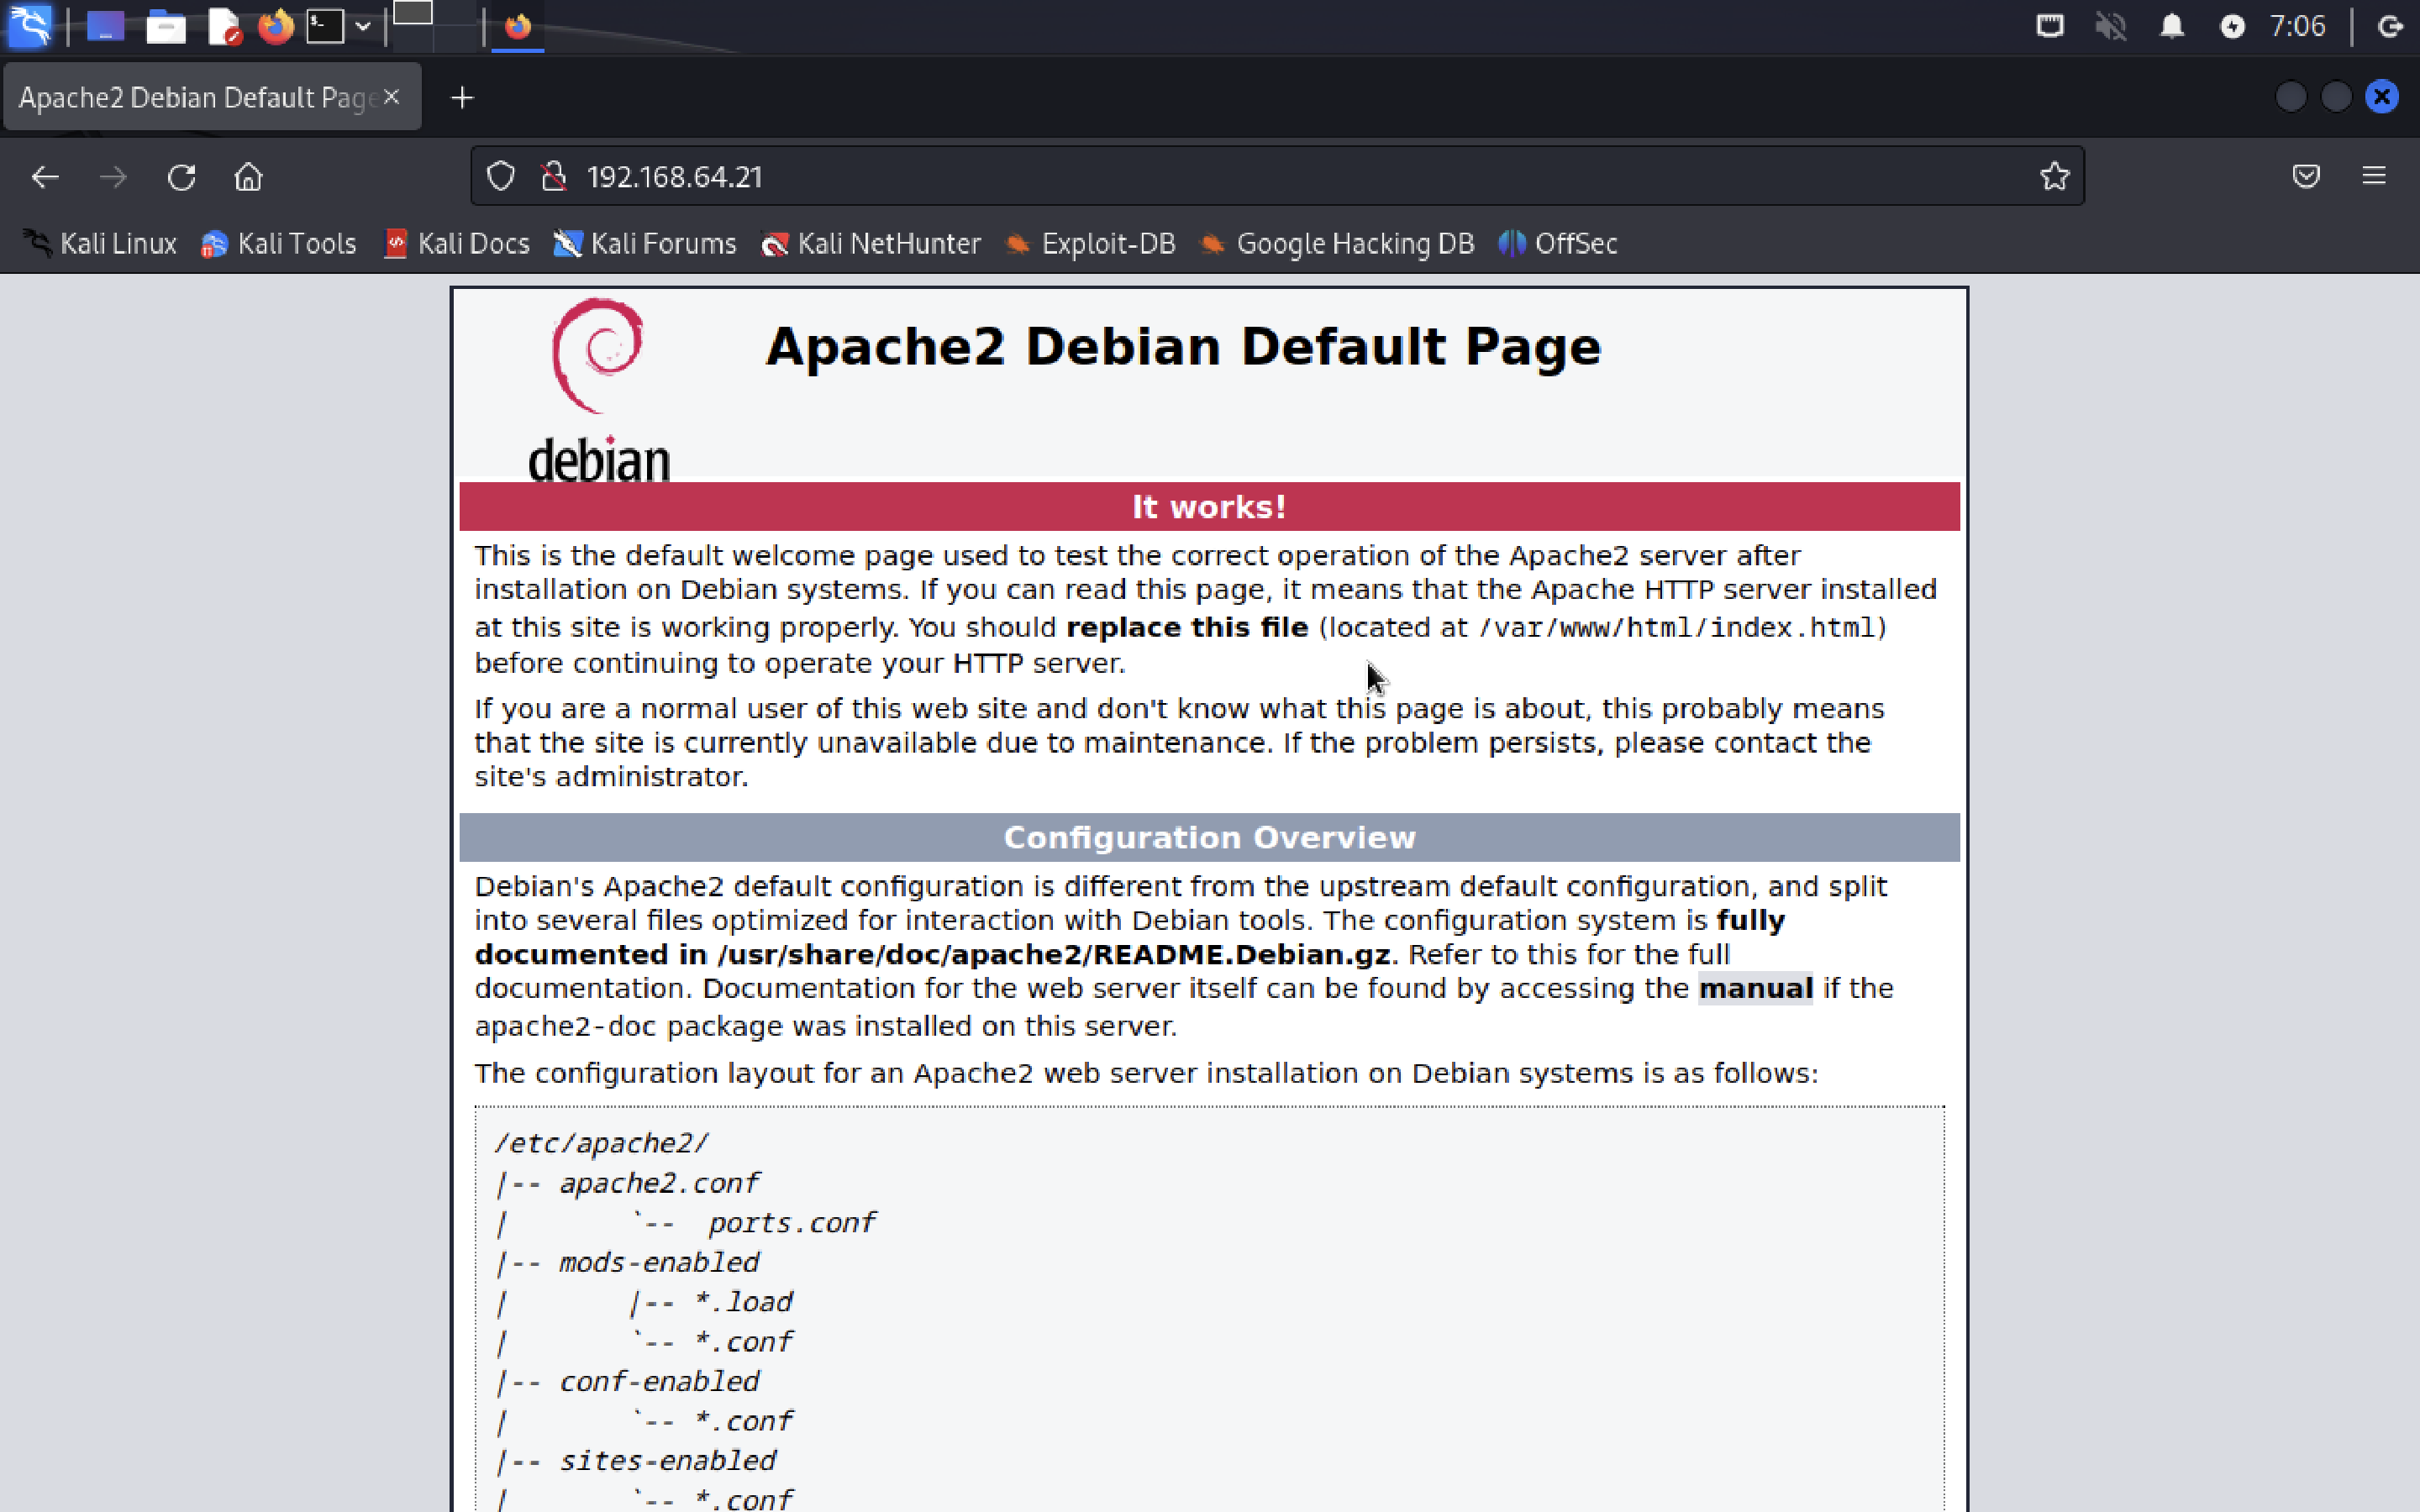
\includegraphics[width=\textwidth]{img/itworks.png}
    \caption{It actually works!}
\end{figure}

Come fase successiva dell'indagine, si è deciso di provvedere alla ricerca dei contenuti presenti sul server web in questione. Allo scopo, saranno utilizzati tre tool in particolare:

\begin{itemize}
    \item \texttt{dirb};
    \item \texttt{dirbuster};
    \item \texttt{gobuster}
\end{itemize}

per ottenere un risultato quanto più preciso possibile. Tutti questi tool fanno riferimento ad un \textbf{dizionario} contenente i nomi delle risorse più comuni presenti sui web server (come directory o file di configurazione).

\newpage
\printbibliography[title={Riferimenti bibliografici e risorse consultate}]
\end{document}